\documentclass{beamer}
\usetheme{owl}           % Use metropolis theme
\newcommand\tab[1][1cm]{\hspace*{#1}}
\title{Proposed Themnothorax decision model (Based on Stephen Pratt \& Mallon et al 2001-2005)}
\date{\today}
\author{Lucas Saldyt}
\institute{Arizona State University}

\usepackage{xcolor}
\usepackage{amsmath}

\makeatletter
\def\mcolor#1#{\@mcolor{#1}}
\def\@mcolor#1#2#3{%
  \protect\leavevmode
  \begingroup
    \color#1{#2}#3%
  \endgroup
}
\makeatother

\newcommand{\annotate}[3]{
\mcolor{#1}{\overbrace{#3}^\text{#2}}
}

\newcommand{\sitem}[1]
{
    \begin{itemize}
        \item #1
    \end{itemize}
}

\bibliographystyle{naturemag}

\definecolor{orange}{HTML}{f7c767}
\definecolor{blue}{HTML}{67E6F7}
\definecolor{green}{HTML}{bdf767}
\definecolor{purple}{HTML}{f467f7}
\definecolor{red}{HTML}{fc4475}
\definecolor{yellow}{HTML}{f4f142}

\usepackage{tikz}
\usetikzlibrary{arrows.meta}

\begin{document}
  \maketitle
  \begin{frame}{Introduction}
      \begin{columns}
          \begin{column}{0.5\textwidth}
              \begin{itemize}
                  \item Temnothorax Albipennis prefers to live in rock crevasses, and emigrates frequently.
                  \item Emigration decision behavior is \mcolor{red}{decentralized, self-organizing, optimal, and error-correcting.}
              \end{itemize}
          \end{column}
          \begin{column}{0.5\textwidth}
               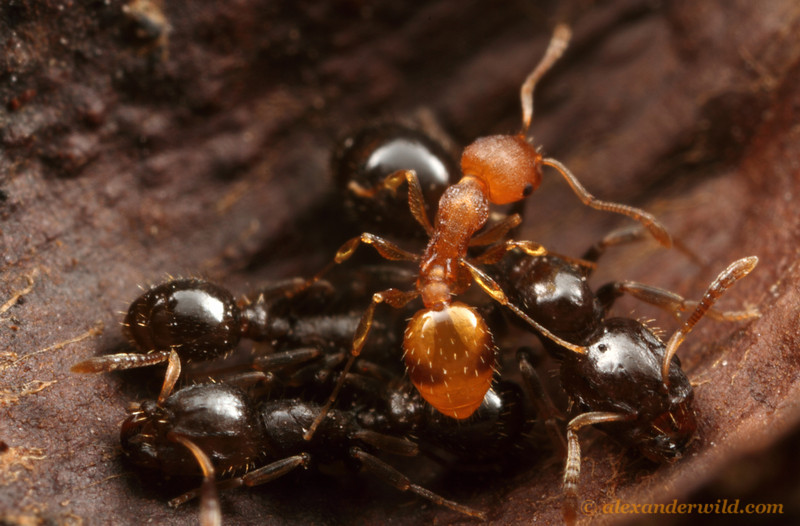
\includegraphics[scale=1.0]{americanus}
          \end{column}
      \end{columns}
  \end{frame}
    \begin{frame}{Legacy Research Questions}
       \begin{itemize}
           \item General: \mcolor{red}{What is responsible for optimal decisions in ant nest choice?}
           \item To what degree is decentralized decision making occuring, and how?
           \item What are the purposes of forward tandem, reverse tandem, and transport?
           \item What is the purpose of quorum, what value is it, and how is it estimated?
       \end{itemize}
   \end{frame}

   \begin{frame}{Overview of Pratt 2002 Equations (Colors showing flow of ant population)}
       \Large
       \begin{equation}
       \begin{aligned}
           & \frac{dS}{dt} = - \sum_{j=1}^M \mcolor{orange}{u_jS} - \sum_{j=1}^M \mcolor{purple}{\lambda_jI(R_j, S)} \\
           & \frac{dA_i}{dt} = \mcolor{orange}{u_iS} + \mcolor{purple}{\lambda_jI(R_j, S)} + \sum_{j \neq i}^M \annotate{blue}{Not meant to be plausible}{(\rho_{ji}A_j - \rho_{ij}A_i)} - \mcolor{green}{k_iA_i} \\
           & \frac{dR_i}{dt} = \mcolor{green}{k_iA_i} + \sum_{j \neq i}^M \annotate{blue}{Not meant to be plausible}{(\rho_{ji}R_j - \rho_{ij}R_i)} \\
           & \frac{dP_i}{dt} = \annotate{red}{Causes overflow if unchecked}{\phi_iJ(R_i, P_0)} - \annotate{white}{Fix: Subtract moved ants}{\phi_{dest}J(R_{dest},P_0)}
       \end{aligned}
       \end{equation}
   \end{frame}

\begin{frame}{The agent based model (Pratt 2005)}
   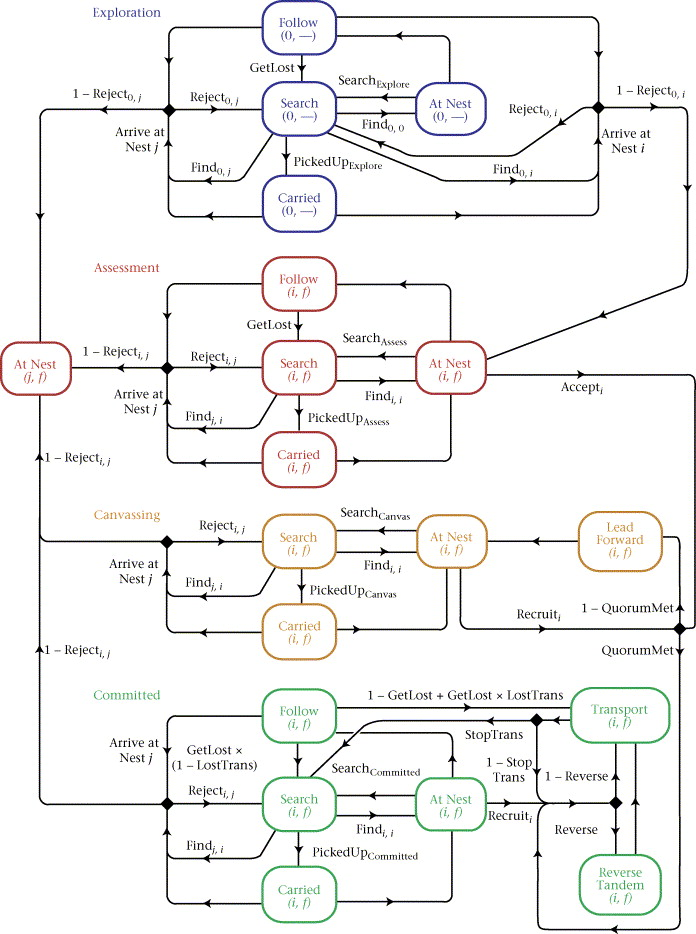
\includegraphics[scale=1.6]{agent}
\end{frame}

\begin{frame}{Model Improvements (1/2)}
  \begin{itemize}
      \item Splitting the \mcolor{red}{$R_i$} population from S. Pratt 2002 into the \mcolor{red}{$L_i$} and \mcolor{red}{$C_i$} populations.
      \item Replacing the two switching equations \mcolor{red}{$I()$} and \mcolor{red}{$J()$} with dynamics switching between \mcolor{red}{$L_i$} and \mcolor{red}{$C_i$} based on a single switching equation \mcolor{red}{$Q()$}.
      \item Fixing unchecked growth in the original \mcolor{red}{$P_i$} equations.
  \end{itemize}
\end{frame}

\begin{frame}{Model Improvements (2/2)}
  \begin{itemize}
      \item Allowing transport of various passive populations, which will allow a split passive population to be fixed.
      \item Replacing switching in \mcolor{red}{$A_i$} and \mcolor{red}{$R_i$} with transitions to searching population. This reflects updates in S.Pratt 2005 and Granovskiy 2012 agent-based models.
      \item Adding transportation of the active population
  \end{itemize}
\end{frame}

\begin{frame}{Proposed Ordinary Differential Equation Model Populations}
  \begin{itemize}
      \item \mcolor{red}{$S$}, searching population
      \item \mcolor{red}{$A_i$}, assessing population at nest $i$
      \item \mcolor{red}{$L_i$}, leading population at nest $i$
      \item \mcolor{red}{$C_i$}, carrying population at nest $i$
      \item \mcolor{red}{$P_i$}, passive population at nest $i$. 
  \end{itemize}
\end{frame}

 
\begin{frame}{Initial Conditions}
    Given \mcolor{red}{$N$} ants, where proportion \mcolor{red}{$p$} are active, the initial states are the following:
   \begin{itemize}
       \item \mcolor{red}{$S = pN$}
       \item \mcolor{red}{$P_0 = (1-p)N$}
       \item \mcolor{red}{$A_i, L_i, C_i, P_i = 0$}
   \end{itemize}
\end{frame}
 
\begin{frame}{Parameters}
    The following table describes the parameters of the model:
 
    \begin{tabular}{ l | c | c | r }
        \hline
      Name          & 2002        & Value & Description (units = rate)\\ \hline
      \mcolor{red}{$\phi_i$}      & $\mu_i$     & 0.13 & Finding nest $i$\\
      \mcolor{red}{$\lambda_i$}   & $\lambda_i$ & 0.033 & Led by leaders to $i$\\
      \mcolor{red}{$\alpha_i$}    & $k_i$       & 0.015, 0.02 & Assessors who accept nest $i$\\ \hline
      \mcolor{red}{$\tau$}        & $\phi_i$    & 0.001  & Uniform transport rate $i$\\
      \mcolor{red}{$\sigma_{Ai}$} & \em{New}    & 0.0195 & Assessing ants enter search from $i$\\
      \mcolor{red}{$\sigma_{Li}$} & \em{New}    & 0.018  & Leading ants enter search from $i$\\
      \mcolor{red}{$\sigma_{Ci}$} & \em{New}    & 0.0044 & Carrying ants enter search from $i$\\
      \hline
    \end{tabular} \\
\end{frame}

\begin{frame}{Parameter Descriptions} 

    \begin{itemize}
        \item \mcolor{red}{$\phi_i$} is the \mcolor{red}{finding} rate for nest  $i$ and is generally uniform.
        \item \mcolor{red}{$\lambda_i$} is the \mcolor{red}{leading} rate for nest $i$ and is generally uniform.
        \item \mcolor{red}{$\alpha_i$} is the \mcolor{red}{accepting} rate for nest $i$. \mcolor{red}{This leads to positive feedback loops, and the equations only work correctly if $\alpha_x > \alpha_y$ for a nest $x$ superior to a nest $y$}
    \end{itemize}
\end{frame}

\begin{frame}{Parameter Descriptions} 
    \begin{itemize}
        \item \mcolor{red}{$\tau$} is a \mcolor{red}{transport} rate, which is the same for all ants

        \item \mcolor{red}{$\sigma_{Xi}$} is a \mcolor{red}{searching} rate where $X$ is each active population ${S, A, L, C}$
    \end{itemize}
\end{frame}

\begin{frame}{Population flow overview}
    \begin{equation}
    \begin{aligned}
         & \frac{dS}{dt} = S * \sum_i \big[\mcolor{orange}{- \phi_i} \mcolor{purple}{- \lambda_iL_i} \mcolor{red}{- \tau C_i} \mcolor{blue}{+ \sigma_{Ai}A_i + \sigma_{Li}L_i + \sigma_{Ci}C_i} \big] \\
         & \frac{dA_i}{dt} = S * [\mcolor{orange}{\phi_i} + \mcolor{purple}{\lambda_iL_i} + \mcolor{red}{\tau \big[ C_i * \sum_{j \neq i}{(S + L_j + C_j + A_j)} - \sum_{j \neq i}{C_j * A_i} \big] } \\ & \mcolor{blue}{- \sigma_{Ai}A_i}] \mcolor{green}{- \alpha_iA_i} \\
        & \frac{dL_i}{dt} = \mcolor{green}{\alpha_iA_i} - \mcolor{yellow}{Q(i)L_i} - \mcolor{red}{\sum_{j \neq i, j} \tau C_jL_i} - \mcolor{blue}{- \sigma_{Ci}C_i} \\
        & \frac{dC_i}{dt} = \mcolor{yellow}{Q(i)L_i} - \mcolor{red}{\sum_{j \neq i, j} \tau C_jC_i} - \mcolor{blue}{- \sigma_{Ci}C_i} \\
        & \frac{dP_i}{dt} = \sum_{j \neq i} [\mcolor{red}{\tau P_j C_i} \mcolor{red}{- \tau P_i C_j}] \\
    \end{aligned}
    \end{equation}

\end{frame}

\begin{frame}{Searching Equation}

%% The following equation describes the searching population, which starts as $Np$.
\begin{multline}
    \frac{dS}{dt} = S * \sum_i \big[\annotate{orange}{Finding nests}{- \phi_i} \annotate{purple}{Led to nests}{- \lambda_iL_i} \annotate{red}{Carried to nests}{- \tau C_i} \\ 
    \annotate{blue}{Began searching from active state}{+ \sigma_{Ai}A_i + \sigma_{Li}L_i + \sigma_{Ci}C_i} \big]
\end{multline}

%% The first term, $\phi_iS$, describes ants that encounter new sites and enter the assessment population.
%% $\lambda_iL_iS$ describes ants being led to new sites and becoming assessors. $L_i$ is included here because the presence of more leading ants will increase the rate at which ants are led to new sites (i.e. ten leading ants lead ants faster than a single ant). Therefore $\lambda_i$ is proportional to $L_i$.
%% $\tau_{Si}C_iS$ describes ants that are transported to new sites. As with the previous term, $\tau_{Si}$ is a rate per individual in $C_i$.
%% Lastly, the $\sigma$ terms describe ants that exit other active states and begin searching, each with an independent rate.

\end{frame}

\begin{frame}{Assessing Equation}
\begin{multline}
\frac{dA_i}{dt} = S * [\annotate{orange}{Found nest i}{\phi_i} + \annotate{purple}{Led to nest i}{\lambda_iL_i} + \annotate{red}{Carried to nest i}{\tau C_i}   
\annotate{blue}{Began searching}{- \sigma_{Ai}A_i}] \\
    \annotate{green}{Accepted nest}{- \alpha_iA_i}
\end{multline}

% The first three terms match the first three terms of the search-population equation.
% $\phi_iS$ describes incoming ants that have found the nest themselves, $\lambda_iL_iS$ describes ants that were carried to the nest $i$, and $\tau_{Si}C_iS$ describes ants that were carried to the nest $i$.
% 
% $\sigma_{Ai}A_i$ describes ants that begin searching after assessing a nest, and lastly $alpha_iA_i$ describes ants that accept a nest and begin recruiting.

\end{frame}

\begin{frame}{Leading Equation}
%% The following equation describes the leading populations, which starts at $0$.

\begin{multline}
    \frac{dL_i}{dt} = \annotate{green}{Accepted nest}{\alpha_iA_i} - \annotate{yellow}{Quorum met}{Q(i)L_i} - \annotate{red}{Transported to nest}{\sum_{j \neq i, j} \tau C_jL_i} \\ 
    - \annotate{blue}{Began searching}{- \sigma_{Li}L_i}
\end{multline}

%% First, the function $Q()$, defined below, returns $1$ if the nest $i$ is above the quorum threshold and $0$ otherwise. Therefore $1 - Q(i)$ is $0$ when the nest is above the quorum threshold and $1$ otherwise.
%% So, when the nest $i$ is above the quorum threshold, only the terms $-Q(i)L_i$ and $\sigma_{Li}L_i$ are active. $Q(i)L_i$ represents a movement of ants from leading to carrying. $\sigma_{Li}L_i$ represents leading ants deciding to enter the search state.
%% When the nest is below the quorum threshold, the first and third term are both active. $1-Q(i)\alpha_iA_i$ describes assessing ants entering the leading populations after accepting a nest, and $1-Q(i)Ci$ describes (potentially) carrying ants reverting to the leading state.
\end{frame}

\begin{frame}{Carrying Equation}
%% The following equation describes the carrying populations, which starts at $0$:

\begin{multline}
    \frac{dC_i}{dt} = \annotate{yellow}{Quorum met}{Q(i)L_i} - \annotate{red}{Transported to nest}{\sum_{j \neq i, j} \tau C_jL_i} \\
    - \annotate{blue}{Began searching}{- \sigma_{Ci}C_i}
\end{multline}

%% Similarly to the leading population equations, $Q()$ acts as a switch. When the nest $i$ is above the quorum threshold, assessing ants will enter the carrying population directly through the $Q(i)alpha_iA_i$ term and leading ants are converted through the $Q(i)L_i$ term.
%% The term $(1-Q(i))C_i$ describes ants that (potentially) revert to the leading state. 
%% Lastly, the term $\sigma{Ci}C_i$ describes ants that enter the searching state from carrying.

\end{frame}

\begin{frame}{Passive Equation}
%% The following equation describes the passive population dynamics. Initially, $P_0 = (1-p)N$ and otherwise $P_i = 0$:
\begin{equation}
\begin{aligned}
    \frac{dP_i}{dt} = \sum_{j \neq i} [\annotate{red}{Ants carried to site i from site j}{\tau P_j C_i} \\ \annotate{red}{Ants carried to site j from site i}{- \tau P_i C_j}]
\end{aligned}
\end{equation}

%% Essentially, the first term $\tau{Pi}P_jC_i$ desribes ants being moved to site $i$ from site $j$, while the second term describes ants being moved from site $i$ to site $j$.
\end{frame}

\begin{frame}{Quorum Function}

%% The $Q()$ switching function is defined as follows, and should be self explanatory. Potentially, (TODO) $P_i$ population should not be counted (but in simulation, this is not a contributing factor):

\begin{equation}
\begin{aligned}
  & Q(i) = 0, \text{if    } \sum [A_i + L_i + C_i] \leq T \\
  & Q(i) = 1, \text{otherwise} \\
\end{aligned}
\end{equation}
\end{frame}

  \begin{frame}{Bibliography}
      \bibliography{sources/insects,sources/brains,sources/ant_system,sources/networks,sources/misc}
  \end{frame}

\end{document}
